\documentclass{article}
\usepackage{amsmath,amssymb,amsthm}
\usepackage{fancyhdr}
\usepackage{enumerate}
\usepackage{graphicx}
\usepackage{caption}
\usepackage{float}
\usepackage{xcolor}

\pagestyle{fancy}
\fancyhf{}
\lhead{2nd Homework - CSCE 312 503}
\rhead{Kevin Lei}
\renewcommand{\headrulewidth}{0.4pt}
\renewcommand{\arraystretch}{1.2}

\definecolor{mygreen}{HTML}{008000}
\definecolor{myorange}{HTML}{d19a02}
\definecolor{myred}{HTML}{b22222}

\begin{document}

\section*{Chapter 4}
\textit{Digital Design, 2nd Ed, by Frank Vahid, Wiley publication, 2010}

\subsection*{4.2}
\begin{figure}[H]
    \centering
    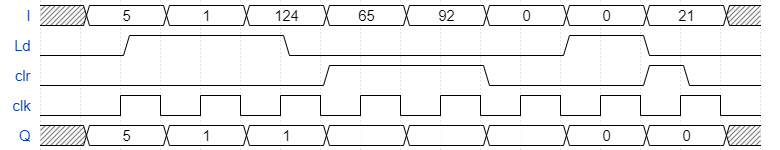
\includegraphics[width=\linewidth]{./images/4.2.png}
    \caption*{Timing diagram parallel load register}
\end{figure}

\subsection*{4.3}
\textbf{Operation table:} \newline
\begin{tabular}{c c | c}
    $S_1$ & $S_0$ & Operation \\
    \hline
    0 & 0 & Maintain \\
    0 & 1 & Parallel load \\
    1 & 0 & Clear \\
    1 & 1 & Complement \\
\end{tabular}

\begin{figure}[H]
    \centering
    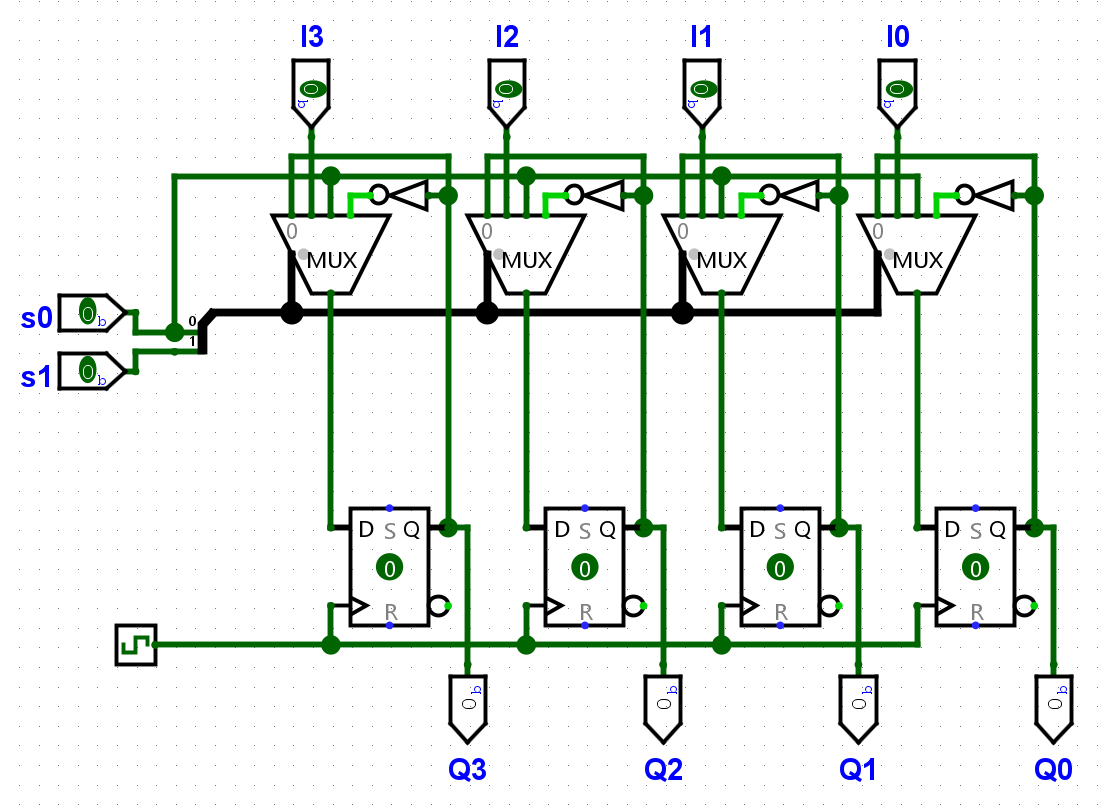
\includegraphics[width=0.9\linewidth]{./images/4.3.png}
    \caption*{Circuit of register}
\end{figure}

\subsection*{4.10}
Assuming the following:
\begin{itemize}
    \item AND gates have a propagation delay of 2ns
    \item OR gates have a propagation delay of 1ns
    \item XOR gates have a propagation delay of 3ns
\end{itemize}
\noindent We want to find the longest propagation delay of an 8-bit ripple-carry adder.
An typical 8-bit ripple-carry adder would use eight full adders.
The total propagation delay would be the sum of the propagation delays of the full adders, since each successive full adder must wait for the carry-out of the previous full adder.
In a typical full adder, the carry-out bit is generated by an AND gate fed into an OR gate.
Thus, the longest propagation delay would be $8 \times (2 + 1) = 24ns$.

\subsection*{4.13}
\begin{figure}[H]
    \centering
    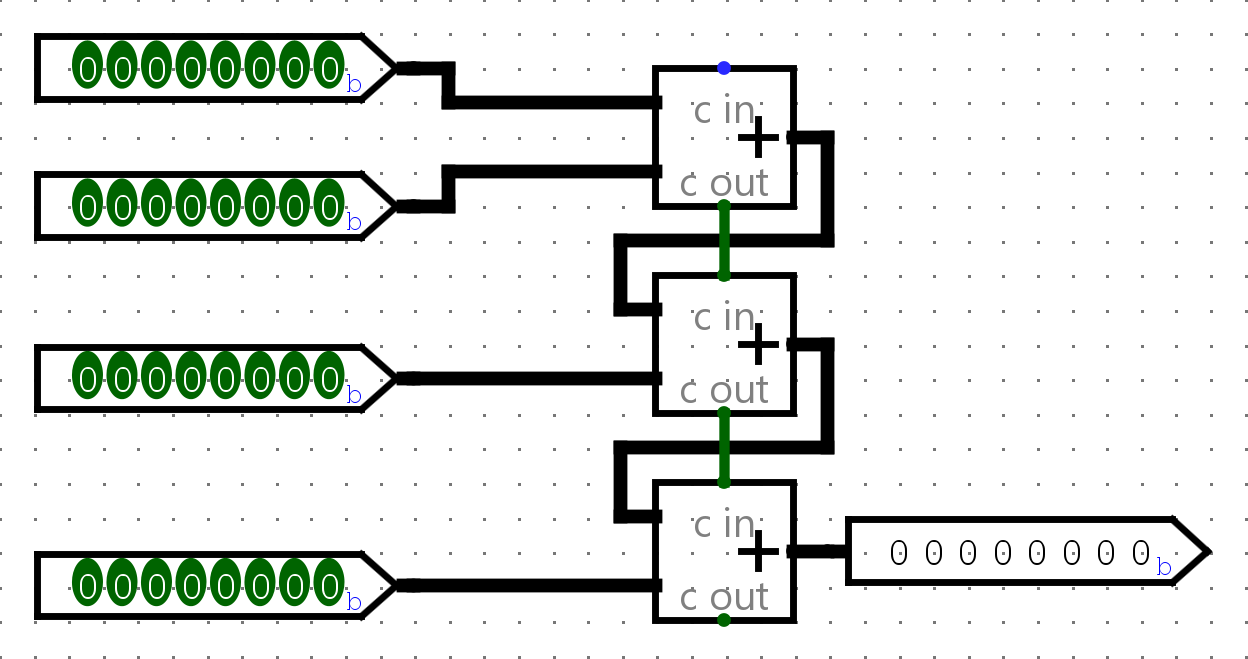
\includegraphics[width=0.9\linewidth]{./images/4.13.png}
    \caption*{Circuit that adds 4 8-bit numbers}
\end{figure}

\subsection*{4.21}
\begin{figure}[H]
    \centering
    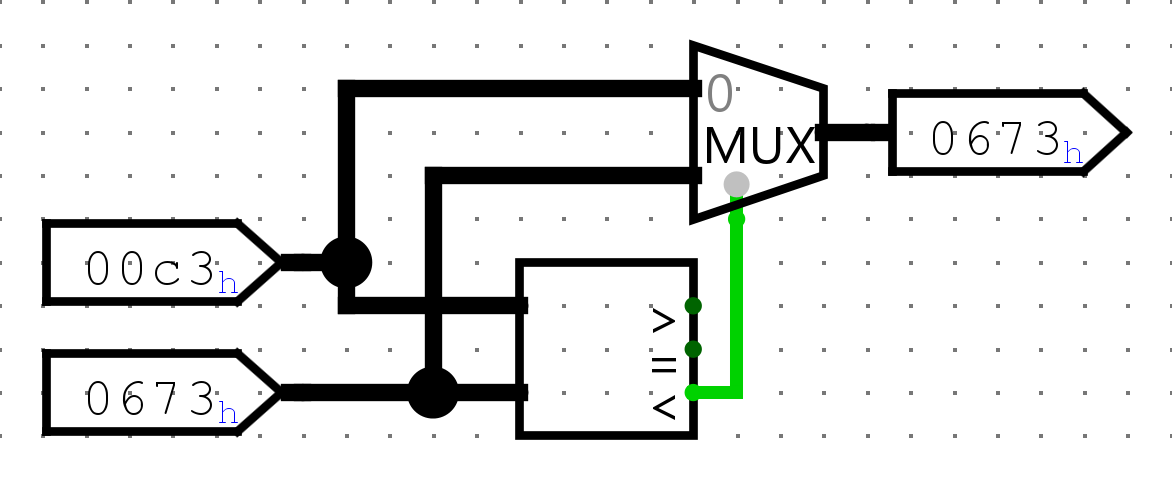
\includegraphics[width=0.9\linewidth]{./images/4.21.png}
    \caption*{Circuit that outputs the greater of two 16-bit numbers}
\end{figure}

\subsection*{4.30}
We can convert two's complement binary to decimal by looking at the most significant bit.
If the most significant bit is 1, then the number is negative, so we first find the magnitude by taking the two's complement.
This is done by inverting all the bits and adding 1.
If the most significant bit is 0, then the number is positive, so we can convert it to decimal directly.
\begin{enumerate}[(a)]
    \item $11100000$ is negative: $00011111 + 1 = 00100000 = 32$
    \item $01111111$ is positive: $2^0 + 2^1 + 2^2 + 2^3 + 2^4 + 2^5 + 2^6 = 127$
    \item $11110000$ is negative: $00001111 + 1 = 00010000 = 16$
    \item $11000000$ is negative: $00111111 + 1 = 01000000 = 64$
    \item $11100000$ is the same as part (a)?
\end{enumerate}

\subsection*{4.33}
To convert from decimal to two's complement binary, we first convert to binary, then take the two's complement if the number is negative.
\begin{enumerate}[(a)]
    \item $29 = 16 + 8 + 4 + 1 = 11101$
    \item $100 = 64 + 32 + 4 = 1100100$
    \item $125 = 64 + 32 + 16 + 8 + 4 + 1 = 1111101$
    \item $-29 = 11101 \rightarrow 00010 + 1 = 00011$
    \item $-100 = 1100100 \rightarrow 0011011 + 1 = 0011100$
    \item $-125 = 1111101 \rightarrow 0000010 + 1 = 0000011$
    \item $-2 = 10 \rightarrow 01 + 1 = 10$
\end{enumerate}

\subsection*{4.40}


\subsection*{4.62}


\subsection*{4.64}


\end{document}